\setcounter{chapter}{6}
\chapter{Mouvement dans un champ uniforme}
\section{Vocabulaire et outils mathématiques}
\subsection{Champ de pesanteur: $\vec{g}$}
\etiquetterouge{Phénomène}  La Terre (comme toutes les grosses masses) crée tout autour d'elle \trou{un champ de pesanteur} que l'on note $\vec{g}$. Lorsqu'une masse $m$ est immergée dans un champ de pesanteur $\vec{g}$ elle subit une force qui vaut $m\times \vec{g}$. Sur Terre, cette force s'appelle aussi le poids et s'écrit: $$\vec{P}=\trou{m.\vec{g}}$$

$\vec{g}$ est vertical, vers le bas et a pour valeur $g=9,8\:m.s^{-2}$.

Lorsqu'en tout point de l'espace $\vec{g}$ garde la même direction, le même sens et la même valeur alors on dit que le champ $\vec{g} $ est \trou{uniforme}.
\paragraph*{Remarque} Dans ce chapitre, le champ de pesanteur est uniforme. 

\subsection{Intégrer une fonction du temps}

\etiquette{Rappel sur la dérivation}

On a vu dans le chapitre précédent, que si on connaît les coordonnées $x(t)$ et $y(t)$ du vecteur position on peut calculer les coordonnées $v_x(t)$ et $v_y(t)$ en utilisant l'opération de \trou{dérivation}.
\\
Par exemple, si $x(t)= -5.t^2 -3t +1$ on  calcule $v_x(t)=\trou{-10t-3}$

\etiquette{Situation} 

Comment faire pour trouver l'expression de $x(t)$ lorsque l'on connaît celle de $v_x(t)$.  On se pose alors la question: "Quelle est la fonction x(t) qui lorsqu'on la dérive donne la fonction $v_x(t)$ ? "\\ On dit que l'on cherche la \trou{primitive de la fonction $v_x(t)$} ou encore que l'on \trou{  intègre  } la fonction $v_x(t)$.

\etiquetterouge{Remarque importante} 

A une fonction $f(t)$ correspond une unique fonction dérivée: $\frac{df(t)}{dt}$ MAIS cette fonction $f(t)$ possède une infinité de primitives. \\ Parmi toutes ces primitives une seule est solution du problème de mécanique étudié\footnote{Pour trouver la "bonne" primitive nous utiliserons des valeurs particulières appelées conditions initiales}.

\etiquetterouge{Primitives à connaître}

\begin{tabular}{l|c}
  $f$ fonction du temps $t$ &Primitive $F(t)$ \\
  \hline \hline 
  $f(t) = 0$ & $F(t)=K$ ; K un réel\\
  \hline
  $f(t) = a$ où a est un réel& $F(t)= a\times t + K$ ; $K$  un réel  \\
  \hline
$f(t)= t$ & $F(t)= \frac{t^2}{2}+ K$ ; K  un réel\\
\hline
$f(t) = a .t + b$ ; a,b deux réels & $F(t)=a.\frac{t^2}{2}+b.t+K$ ; K un réel\\
\hline
\end{tabular}

\etiquette{Application immédiate}
Pour chaque cas, proposer une fonction $x(t)$ qui est une primitive de la fonction $v_x(t)$
\begin{itemize}
	\item $v_x(t) = 5$
	\item $v_x(t)= t$
	\item $v_x(t) = 2t-3$
\end{itemize}


\section{Mouvement dans un champ de pesanteur uniforme}
\subsection{Objectifs}
Nous allons étudier 3 cas: 
\begin{enumerate}
	\item Chute libre sans vitesse initiale.
	\item Chute libre avec une vitesse initiale horizontale.
	\item Chute libre avec une vitesse initiale oblique.
\end{enumerate}

\etiquetterouge{Faites attention à}
	\begin{itemize}
		\item L'enchaînement des étapes qui permettent de passer du bilan des forces aux équations horaires.
		\item Aux conditions initiales, leurs écritures mathématiques et comment elles permettent de déterminer les constantes d'intégration.
	\end{itemize}

\subsection{Chute libre sans vitesse initiale}

\etiquette{Description} 
On lâche à l'instant $\rm t=\SI{0}{\second}$ une bille de masse $\rm m=\SI{100}{\gram}$ d'une hauteur $ \rm h= \SI{5,00}{\meter}$. On notera $\rm \overrightarrow{OM}(t)$ le vecteur position de la bille à chaque instant t.
On note x(t) et y(t) les coordonnées de la bille. 

Les conditions initiales sont $x(0)=0$ ; $y(0)=h=5$ m ; $v_x(0)=v_y(0)=0$ m/s

\includegraphics{figures/dynamique/chute1}


\begin{enumerate}
\item
Faire le bilan des forces exercées sur la bille au cours de la descente.
\item Ecrire la seconde loi de Newton.
\item En déduire les coordonnées du vecteur accélération à l'instant t.
\item En déduire les coordonnées du vecteur vitesse $\overrightarrow{v}(t)$.
\item En déduire les coordonnées du vecteur position $\rm \overrightarrow{OM}(t)$.
\item Le mouvement dépend-il de la masse ? 
\item À quel instant la bille touche-t-elle le sol ? Avec quelle vitesse ?
\end{enumerate}

\subsection{Chute libre avec vitesse initiale horizontale}
\etiquette{Description} On considère une bille M de masse $\rm m=\SI{100}{\gram}$ dont les coordonnées sont notées x(t), y(t) et z(t) à chaque instant. On lance horizontalement à $\rm t=\SI{0}{\second}$ la bille de telle manière que $\rm x(0)=\SI{0}{\meter}$ ; $\rm y(0)=\SI{5}{\meter}$ ; $\rm z(0)=\SI{0}{\meter}$ \\ $\rm v_x(0)=\SI{3}{\meter\per\second}$ ;  $\rm v_y(0)=\SI{0}{\meter\per\second}$ et $\rm v_z(0)=\SI{0}{\meter\per\second}$ 

\includegraphics{figures/dynamique/chute2}


\begin{enumerate}
\item Représentez l'allure de la trajectoire (sans calculs).
\item La vitesse suivant l'horizontale va-t-elle augmenter, diminuer, ou rester constante ?
\item La vitesse suivant la verticale va-t-elle augmenter, diminuer, ou rester constante ?
\item
Faire le bilan des forces exercées sur la bille au cours de la descente.
\item En déduire les coordonnées du vecteur accélération à l'instant t.
\item En déduire les coordonnées du vecteur vitesse $\overrightarrow{v}(t)$.
\item Le mouvement est-il plan ? Justifier.
\item En déduire les coordonnées du vecteur position $\rm \overrightarrow{OM}(t)$.
\item Déterminer l'équation de la trajectoire.
\item À quel instant la bille touche-t-elle le sol ? Avec quelle vitesse ?
Comparer votre résultat à la situation précédente (sans vitesse initiale).
\end{enumerate}

\newpage
\subsection{Le tir parabolique}

\etiquette{Description} On lance une balle selon une direction faisant un angle $\alpha=\SI{60}{\degree}$ avec l'horizontale, avec une vitesse initiale dont la valeur est  $v_0=2\:m /s$. A t=0 s, la balle se situe au niveau du sol, au point O.

\includegraphics{figures/dynamique/chute3}

\begin{enumerate}
\item Faire le bilan des forces exercées sur la bille au cours du mouvement.
\item En déduire les coordonnées du vecteur accélération à l'instant t.
\item En déduire les coordonnées du vecteur vitesse $\overrightarrow{v}(t)$.
\item La vitesse suivant l'horizontale va-t-elle augmenter, diminuer, ou rester constante ? Faire le lien avec le bilan des forces.
\item La vitesse suivant la verticale va-t-elle augmenter, diminuer, ou rester constante ? Faire le lien avec le bilan des forces.
\item En déduire les coordonnées du vecteur position $\rm \overrightarrow{OM}(t)$.
\item Le mouvement est-il plan ? Justifier.
\item Déterminer l'équation de la trajectoire 
\item Déterminer l'abscisse du point d'impact lorsque la balle touche le sol.
\end{enumerate}

\blocrouge{Travail personnel}{
\begin{itemize}
	\item Refaire régulièrement les exemples précédents (faire ses gammes...)
	\item Ex 13 p 252 pour projeter $\vec{v_0}$
	\item Revoir les techniques:  10  ,18 et 28 p 250 et suivantes (calculs classiques)
	\item Préparer le contrôle: 30 p 255
	\item Sujet type bac: Métropole juin 2021 sujet 2 Exercice A question 1 à 5
	\item Sujet bac: Métropole SI 2022 septembre Jour 1 "Etude d'une frappe au football"
	\item Sujet bac: Asie 2021 jour 2 "Water bottle flip"
\end{itemize}}
\newpage
\section{Aspect énergétique}
\subsection{Rappels}
\blocgris{Formules à connaître}{
\begin{itemize}
	\item Energie potentielle de pesanteur: $$Ep=\trou{mgz}$$ \\ $z$ est l'altitude\footnote{On suppose que l'on dispose d'un axe (Oz) verticale orientée positivement vers le O qui permet de repérer l'altitude du système} en mètre du système.
	\item Energie cinétique:$$Ec=\trou{\frac{1}{2}mv^2}$$\\ $v$ la vitesse du système en m/s. 
	\item Energie mécanique:$$Em=\trou{Ec+Ep}$$\\ Les énergies Ep, Ec et Em s'expriment en joules dont le symbole est J. C'est l'unité légale de mesure de l'énergie.
\end{itemize}
}

\blocrouge{Conservation de l'Em}{Si le système n'est soumis qu'à des forces conservatives (comme le poids ou la force électrique) alors son énergie mécanique reste constante. Cela signifie que pour deux instants $t_1$ et $t_2$ on a: $$Em(t_1) = Em(t_2)$$ } 

\paragraph*{Remarque} Les forces de frottements ne sont pas des forces conservatives. Si un système subit des frottements alors \trou{son énergie mécanique sera décroissante au cours du temps}.
\subsection{Etude énergétique d'une chute libre}
On se place dans le cas d'une balle lâchée (sans vitesse initiale)  d'une hauteur  $h=5$ m. A l'instant $t_1=0$ s, la balle est lâchée et à l'instant $t_2$ elle touche le sol.

\etiquetterouge{Objectif} 

Nous allons faire un bilan d'énergie mécanique entre l'instant initial $t_1$ et l'instant $t_2$ où elle atteint le sol. Nous en déduirons la vitesse de la balle à l'instant $t_2$ (moment de l'impact au sol).

\etiquette{Travail}

\begin{enumerate}
\item Rappeler l'expression de la vitesse de la balle au moment où elle touche le sol.
\item Calculer à $t_1$=0 s l'énergie cinétique et potentielle du système. En déduire la valeur initiale de l'énergie mécanique.
\item A l'instant $t_2$, donner l'expression littérale de l'énergie cinétique ? Que vaut l'énergie potentielle à cet instant ?
\item En utilisant la conservation de l'énergie mécanique et les questions précédentes déduire l'expression littérale de la vitesse de la balle à l'instant $t_2$. Faire l'application numérique.
\end{enumerate}

\blocrouge{Travail personnel}{
\begin{itemize}
	\item Ex 1 p 248  et 21 p 253 (énergie mécanique)
	\item Sujet BAC: 2021 Métropole septembre Exercice C: Cesta Punta partie 2
	\item Exercice A: Saut à l'élastique: \url{https://www.labolycee.org/sujets-2-bac-metropole-juin-2021}
	\item Travail de la force électrique BAC 2022 \url{https://www.labolycee.org/impression-3d-dobjets-metalliques}
\end{itemize}
}


\section{Mouvement dans un champ électrique uniforme}
\subsection{Charge électrique $q$}
Certaines particules possèdent une charge électrique que l'on note $q$ et qui se mesure en \trou{coulomb noté: C}.
La plus petite charge électrique s'appelle \trou{la charge élémentaire}, c'est aussi la charge d'un proton. Elle se note $e$ et vaut $$e=\trou{\SI{1.6e-19}{\coulomb}}$$
Par exemple:
\begin{itemize}
	\item la charge de l'électron vaut: $q= -\SI{1.6e-19}{\coulomb}$.  
	\item La charge d'un ion $Cu^{2+}$ vaut $q = 2 \times e = \SI{3.2e-19}{\coulomb}$

\end{itemize}

\etiquetterouge{Phénomène} 
Toute charge électrique crée autour d'elle un champ électrique: $\vec{E}$. Ce champ est représenté par un vecteur dont la valeur s'exprime en \trou{V/m}.


\vspace{1cm}

\includegraphics[width=4cm]{figures/dynamique/chargemoins.png}
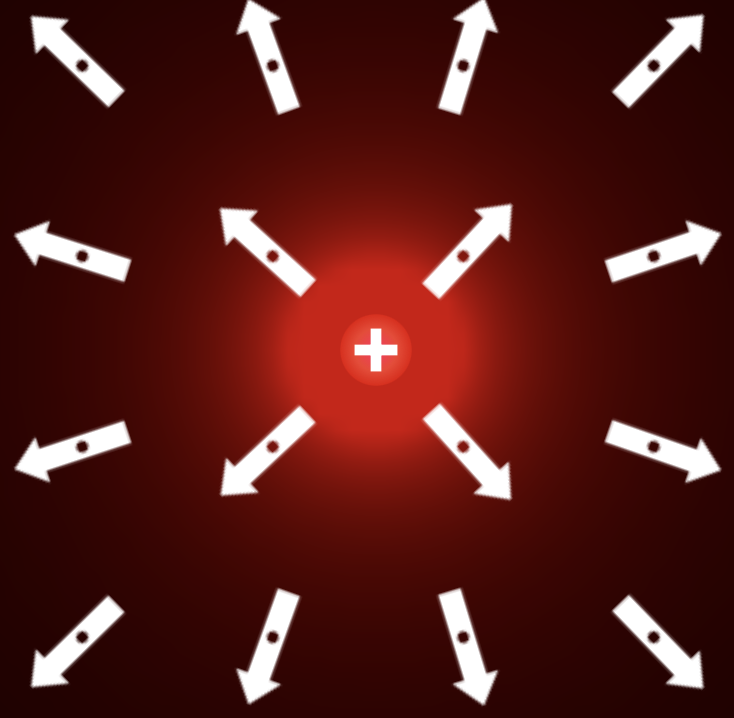
\includegraphics[width=4cm]{figures/dynamique/chargeplus.png}
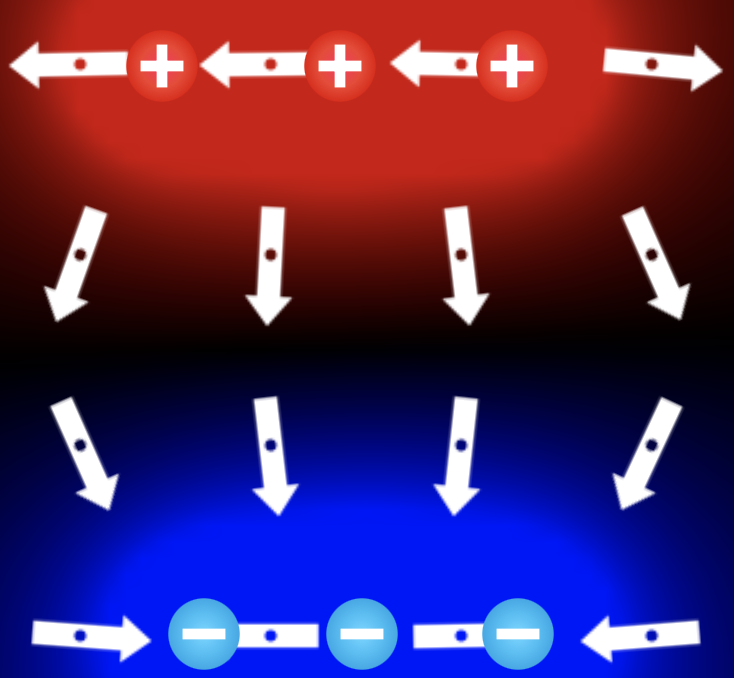
\includegraphics[width=4cm]{figures/dynamique/champ_plaques.png}

\subsection{Champ électrique à l'intérieur de deux plaques chargées}


\etiquette{Situation} On soumet deux plaques métalliques séparées d'une distance $d$ à une tension électrique U imposée par un générateur. Entre ces deux plaques apparaît un champ électrique $\vec{E}$.

A la manière du champ de pesanteur $\vec{g}$, le champ électrique est uniforme (dans la zone entre les plaques) car ses caractéristiques restent les mêmes en tout points. 

\etiquette{Schéma}

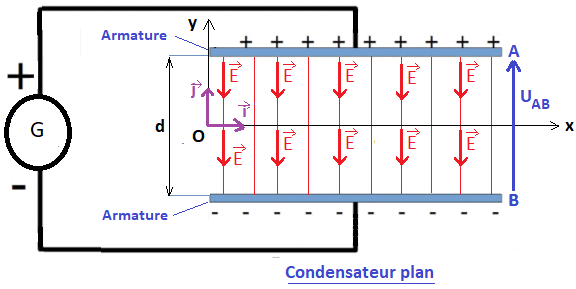
\includegraphics[width=12cm]{figures/dynamique/champ_plaques_2.png}

\blocrouge{Caractéristiques de $\vec{E}$}{
\begin{itemize}
	\item Direction: $\vec{E}$ est  perpendiculaire aux plaques
	\item Sens: orienté de la plaque + vers la plaque -
	\item Valeur: $$E=\trou{\frac{U_{AB}}{d}}$$ Avec $U_{AB}=V_A-V_B$ 
\end{itemize}
E en V/m ; $U_{AB}$ en V et d en m 
}
\etiquette{Calcul de l'intensité du champ électrique}

Le générateur applique une tension de 500 V. Les plaques sont distantes de 5 cm. Calculer la valeur du champ électrique E.







\subsection{Force électrique }

\etiquetterouge{Phénomène} Lorsqu'une charge $q$ est plongée dans un champ électrique $\vec{E}$ elle subit une force $\vec{F}$ qui s'écrit$$\vec{F} = \trou{q\times \vec{E}}$$

\textbf{Attention} Si $q>0$ la force et le champ électrique sont de même sens mais si $q<0$ la force est de sens opposé à $\vec{E}$.
\etiquette{Représentation de $\vec{F}$}

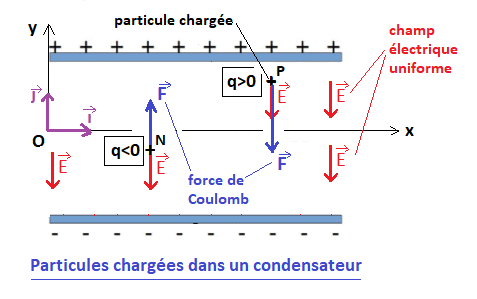
\includegraphics[scale=0.7]{figures/dynamique/force_electrique}

Simulation: \url{https://dlatreyte.github.io/terminales-pc/chap-8/5-mouvement-champ-electrique/}
\etiquette{Application immédiate }
\begin{enumerate}
	\item Représenter, sur les schémas ci-dessous, qualitativement, les charges sur les plaques ou la trajectoire de la particule q.
	\item Sur chaque schéma, représenter $\vec{F}$ et $\vec{E}$

\end{enumerate}

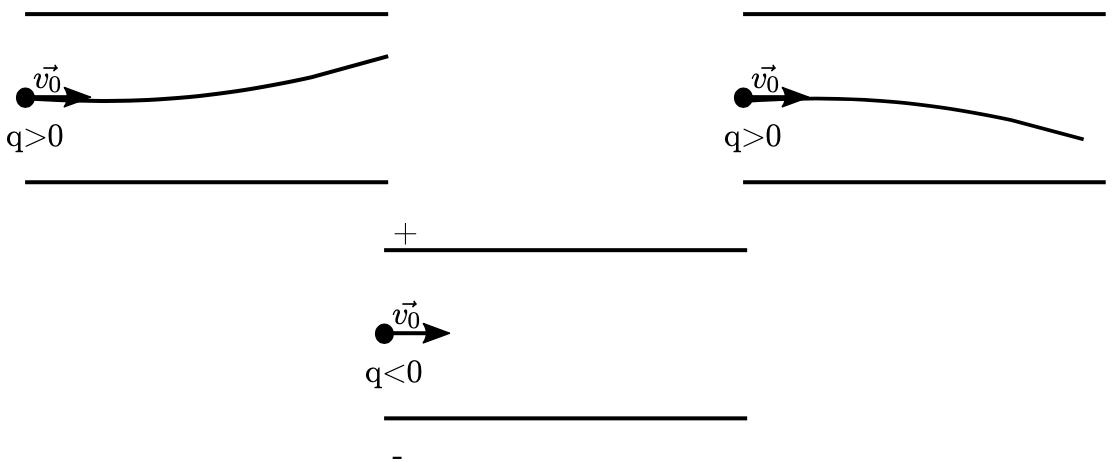
\includegraphics[width=0.8\textwidth]{figures/dynamique/etude_cas}
\newpage
\etiquette{Exercice classique 1}

\begin{minipage}{.50\textwidth}
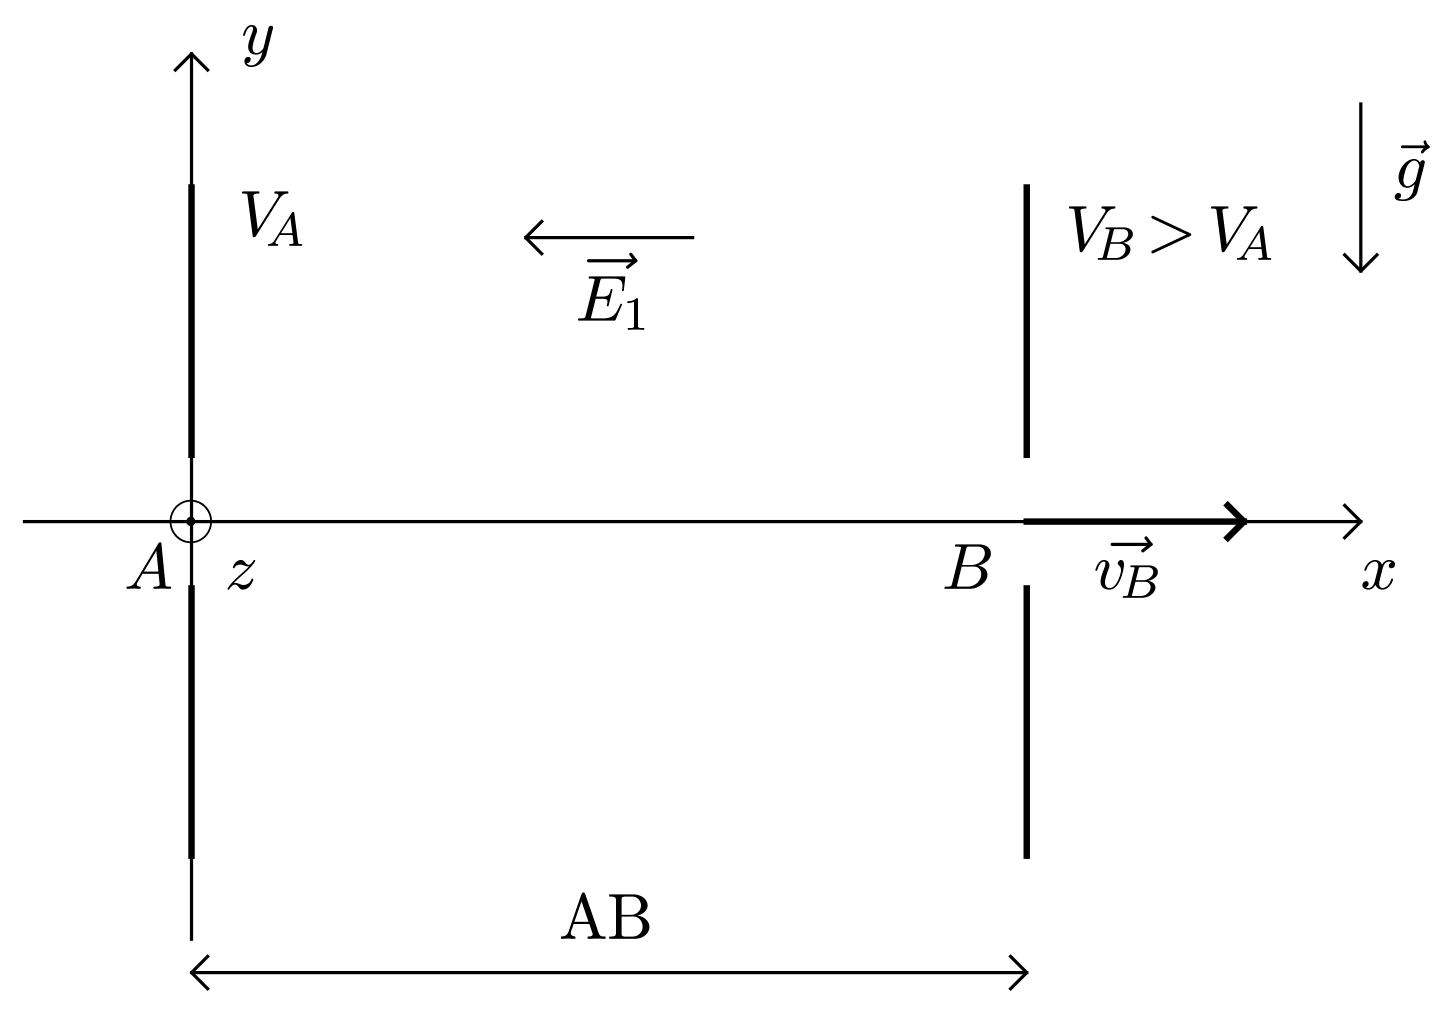
\includegraphics[width=1\textwidth]{figures/dynamique/Chap-8-5-5}  
\end{minipage}
\hfill
\begin{minipage}{.45\textwidth}
Un électron est produit avec une vitesse nulle au point A  entrée d'une zone de l'espace où règne un champ électrique $\vec{E}_{1}$ créé par deux armatures conductrices planes parallèles distantes de AB et le champ de pesanteur $\vec{g}$. On Cherche à déterminer les équations horaires du mouvement de l'électron et plus particulièrement sa vitesse $\vec{v}_{B}$  au point B.\\ \textbf{Données}\
e=\SI{1,6e-19}{C} \\  $m_e$= \SI{9,11e-31}{kg} ; AB= 3 cm ; $E_1$= \SI{6,0e4}{V/m}
\end{minipage}
\paragraph*{Calcul de $v_B$ à partir de la seconde loi de Newton}
\begin{enumerate}
	\item Déterminer les interactions auxquelles est soumis l'électron. 
	\item Ecrire la seconde loi de Newton.
	\item Calculer la valeur de la force électrique puis celle du poids. En déduire que l'on peut négliger dans la suite le poids.
	\item Déterminer les coordonnées du vecteur accélération, vitesse et position. 
	\item Déterminer la valeur de la vitesse en B.
\end{enumerate}


\etiquette{Exercice classique 2}

\begin{minipage}{.50\textwidth}
  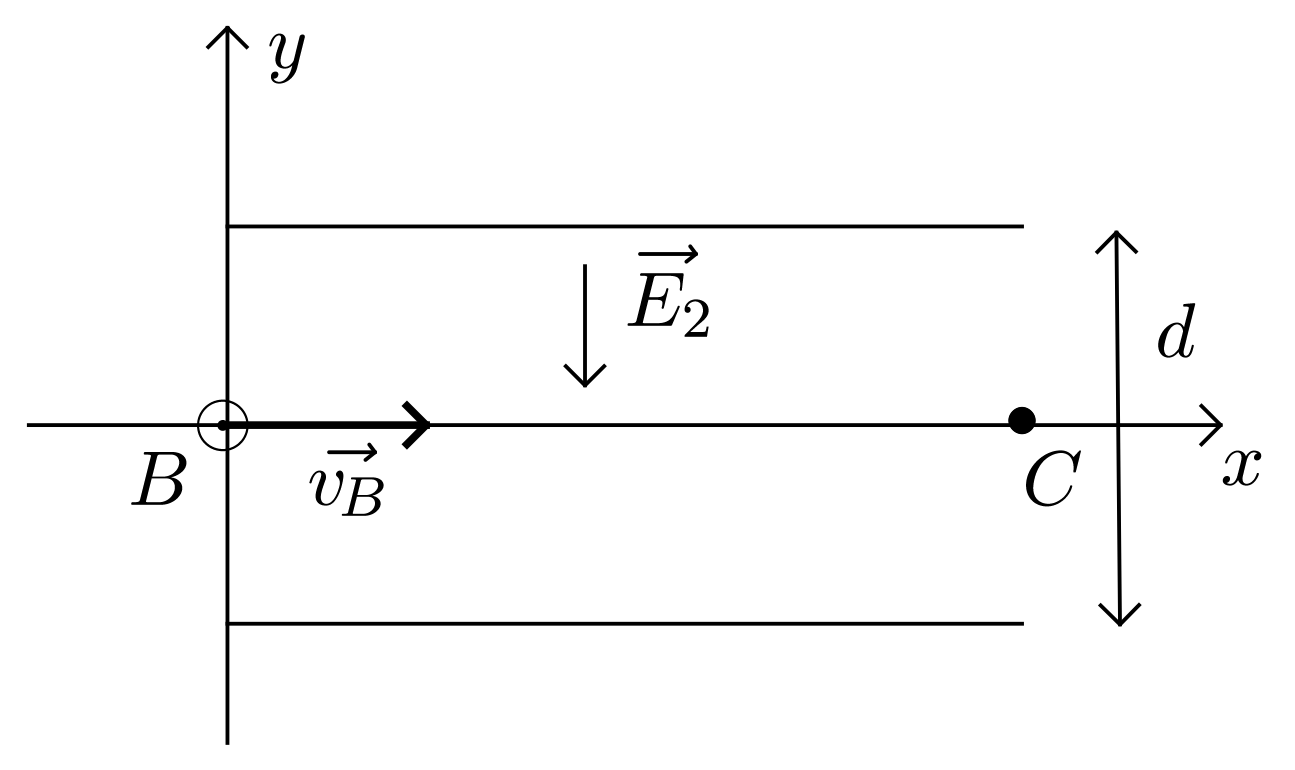
\includegraphics[width=.9\textwidth]{figures/dynamique/Chap-8-5-9}
\end{minipage}
\hfill
\begin{minipage}{.45\textwidth}
  L'électron entre maintenant dans une nouvelle zone dans laquelle règne un champ électrique $\vec{E_2}$ avec la vitesse $\vec{v_B}$ déterminée dans la section précédente.
  A t=0 l'électron est en B.
  
  \textbf{Données}\
BC=6,0 cm ; d= 3 cm ; $E_2$= \SI{1,0e14}{V/m}
\end{minipage}

\begin{enumerate}
	\item Appliquer la seconde loi de Newton et déterminer les coordonnées des vecteurs: accélération, vitesse et position en tenant compte des conditions initiales.
	\item Etablir l'équation de la trajectoire lorsque l'électron est soumis à $\vec{E_2}$.
	\item Déterminer les expressions des coordonnées du point de sortie de l'électron.
	\item Quel  est le mouvement de l'électron lorsqu'il a quitté les deux zones dans lesquelles règnent les champs électriques $\vec{E_1}$  et $\vec{E_2}$ ?
\end{enumerate}

\blocrouge{Travail personnel}{
\begin{itemize}
	\item Ex 11 et 19 p 251 et suivantes 
	\item 33, 34 p 256-257
\end{itemize}

 }
%
%\subsection{Etude du Mouvement d'une charge $q$ dans un $\vec{E}$}
%
%\begin{enumerate}
%\item
%Représenter sur la figure 1 le champ électrique au point O\\
%
%\begin{figure}[htp!]
%\begin{center}
%%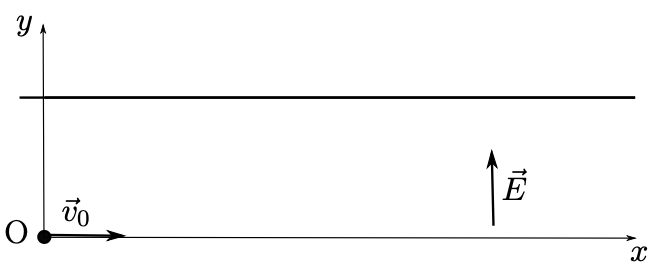
\includegraphics[scale=0.6]{figures/dynamique/fig_exo.png}	
%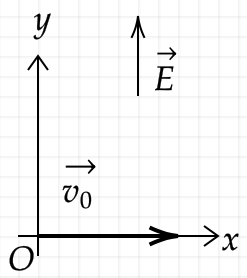
\includegraphics[scale=0.4]{figures/dynamique/mouvement_charge_electrique.png}	
%\end{center}
%\caption{Mouvement d'un électron dans un champ électrique uniforme}
%\end{figure}
%\end{enumerate}
%
%Un électron arrive au point O avec une vitesse initiale $\vec{v}_0$.
%
%\begin{enumerate}
%\stepcounter{enumi}
%\item Exprimer la force $\vec F$ subie par l'électron soumis au champ $\vec E$.
%\item Représenter qualitativement cette force sur la figure 1.
%\item Représenter sur la figure 1  l'allure de la trajectoire de l'électron (sans calculs).
%\item Appliquer la deuxième loi de Newton à l'électron sachant que le poids est une force négligeable devant $\vec F$.
%\item En déduire les coordonnées du vecteur accélération $\vec a$ à un instant t.
%\item En déduire les coordonnées du vecteur vitesse $\vec v$ à un instant t.
%\item En déduire les coordonnées du vecteur position $\vec{OM}$ à un instant t.
%\item Déterminer l'équation de la trajectoire.
%\end{enumerate}
%
%\etiquettebleue{Application numérique} Un faisceau d'ions oxyde $O^{2-}$ est envoyé dans un condensateur plan de longueur $L=\SI{10}{\centi\meter}$ où règne un champ électrique de valeur $E=\SI{100}{\kilo\volt\per\meter}$.\\
%La valeur initiale de la vitesse de chaque ion est $v_0=\SI{5,0e5}{\meter\per\second}$.\\
%Déterminer l'ordonnée de sortie des ions selon qu'ils appartiennent à l'isotope 16 ou à l'isotope 18 de l'oxygène, de masses respectives $m_{16}=\SI{2,66e-26}{\kilo\gram}$ et $m_{18}=\SI{2,99e-26}{\kilo\gram}$.

